\documentclass{article}%
\usepackage[T1]{fontenc}%
\usepackage[utf8]{inputenc}%
\usepackage{lmodern}%
\usepackage{textcomp}%
\usepackage{lastpage}%
\usepackage[head=40pt,margin=0.5in,bottom=0.6in]{geometry}%
\usepackage{graphicx}%
%
\title{\textbf{Ana María Dacosta denunció tortura contra Jofran Quintero}}%
\author{EL NACIONAL WEB}%
\date{03/12/2018}%
%
\begin{document}%
\normalsize%
\maketitle%
\textbf{URL: }%
http://www.el{-}nacional.com/noticias/presos{-}politicos/ana{-}maria{-}dacosta{-}denuncio{-}tortura{-}contra{-}jofran{-}quintero\_261934\newline%
%
\textbf{Periodico: }%
EN, %
ID: %
261934, %
Seccion: %
Presos políticos\newline%
%
\textbf{Palabras Claves: }%
Política, Presos políticos\newline%
%
\textbf{Derecho: }%
1.3%
, Otros Derechos: %
1.2%
, Sub Derechos: %
1.3.1, 1.2.2%
\newline%
%
\textbf{EP: }%
NO\newline%
\newline%
%
\textbf{\textit{La activista política aseguró que Quintero presenta lesiones en la cara, en la cabeza y en el cuello. Asimismo, responsabilizó a Nicolás Maduro y Néstor Reverol por la integridad del preso político}}%
\newline%
\newline%
%
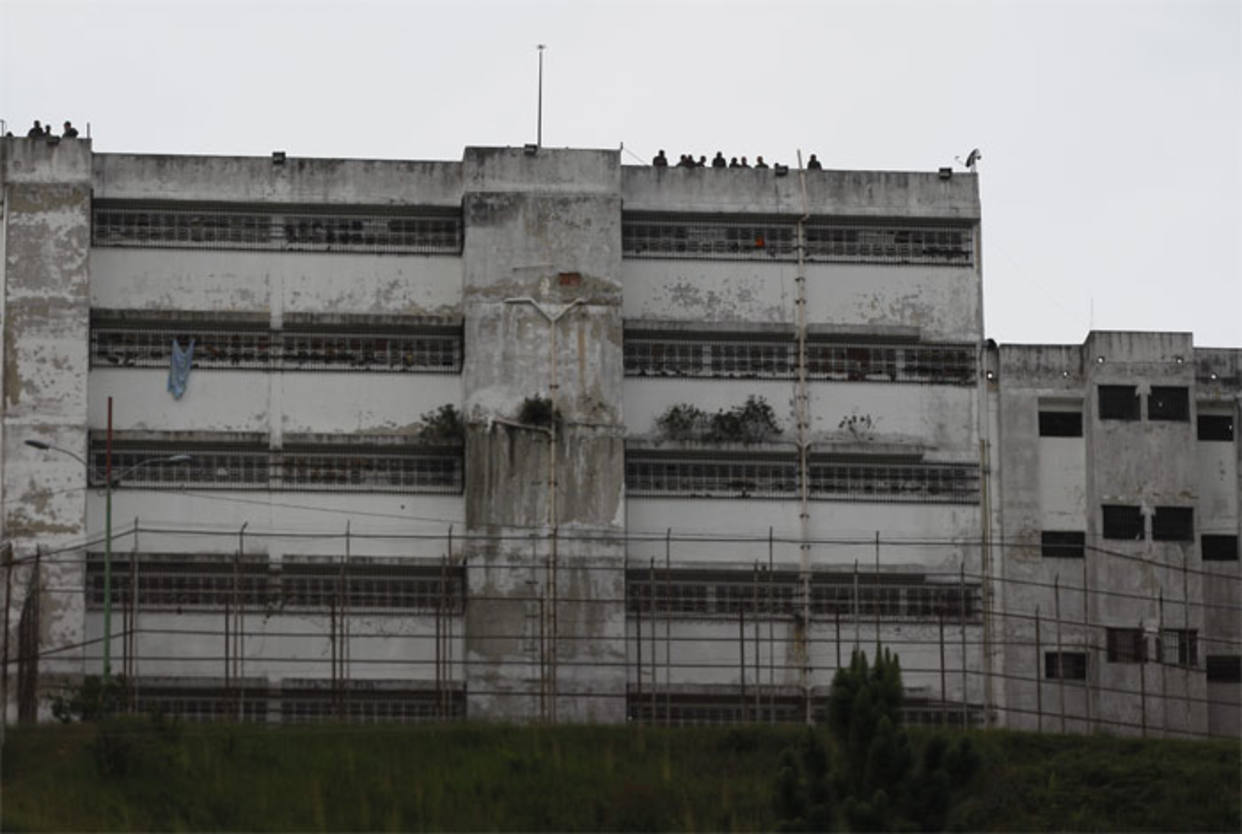
\includegraphics[width=300px]{14.jpg}%
\newline%
%
Ana María Dacosta, activista y hermana del preso político Vasco Dacosta, denunció que durante su visita a la cárcel de Ramo Verde pudo constatar que Jofran Quintero presentaba signos de golpes y torturas físicas.%
\newline%
%
“Estaba fuertemente golpeado, con hematomas en la cara, en la cabeza y en el cuello. Presenta un gran dolor en las costillas que le impide respirar bien”, expresó la activista mediante un video compartido en Twitter.%
\newline%
%
Da~Costa responsabilizó a Nicolás Maduro y Néstor Reverol por la integridad física de Quintero.%
\newline%
%
\end{document}